%Once subsystems are chosen, they need to be integrated. Each specialized system was built independently and provides it?s own query language (SQL, CQL, HiveQL, pig, N1QL, MongoDB...) and data model (relational, semi-structured, graph, key-value...). Yet a single query interface, common query language and common data model are required. The common query language and data model need to be as expressive as any of the query languages of the subsystems, in order to leverage fully the expressive power of every subsystem.

\subsection{Integrating data from multiple sources : historical review}

The goal of a PP system is to provide an unique query interface to interact with the various subsystems it provides. These subsystems each have their own The problem of integrating data coming from multiple sources is a classical problem in data integration which has been extensively studied ~\cite{Lenzerini2002}. 

Federated Query Processor MiddleWare Architecture

Most PP systems that have been studied focus on middle ware based architecture in which the user specifies a query which is then translated into sub components.

Each sub component corresponding to a fragment which is sent to individual subsystems.

These fragments are then translated into the subsystem's native query language and executed on those subsystems.

The results of the fragment queries are then returned to the middleware which joins them together to form a response to the user initial query.

This technique is inherited from the classical data integration integration problem that has been studied extensively in the 1990's.

Describe first what is the global as view approach 

\subsection{Finding a unifying data model and query language}

\subsubsection{procedural vs declarative approach}

Relevant papers : ~\cite{Lenzerini2002} ~\cite{Kirk1995} ~\cite{Katsis2009}
~\cite{Srivastava2006} ~\cite{Tatbul2010} ~\cite{Botan2009} ~\cite{Botan2010} ~\cite{Lim2013}
~\cite{Sharp2013} ~\cite{Cure2011} ~\cite{Atzeni2012} ~\cite{Sellami2014} ~\cite{Sellami2013}
~\cite{Ong2014} ~\cite{Ong2015} ~\cite{Boag2010} ~\cite{Ives2002} ~\cite{Borkar2006}
~\cite{Liu2010} ~\cite{Fowler2012}

 \reminder{Jules : In this section, we show what the generic, classical middleware query architecture looks like with the databases chosen above.}
 
 
\begin{figure}
 \centering
  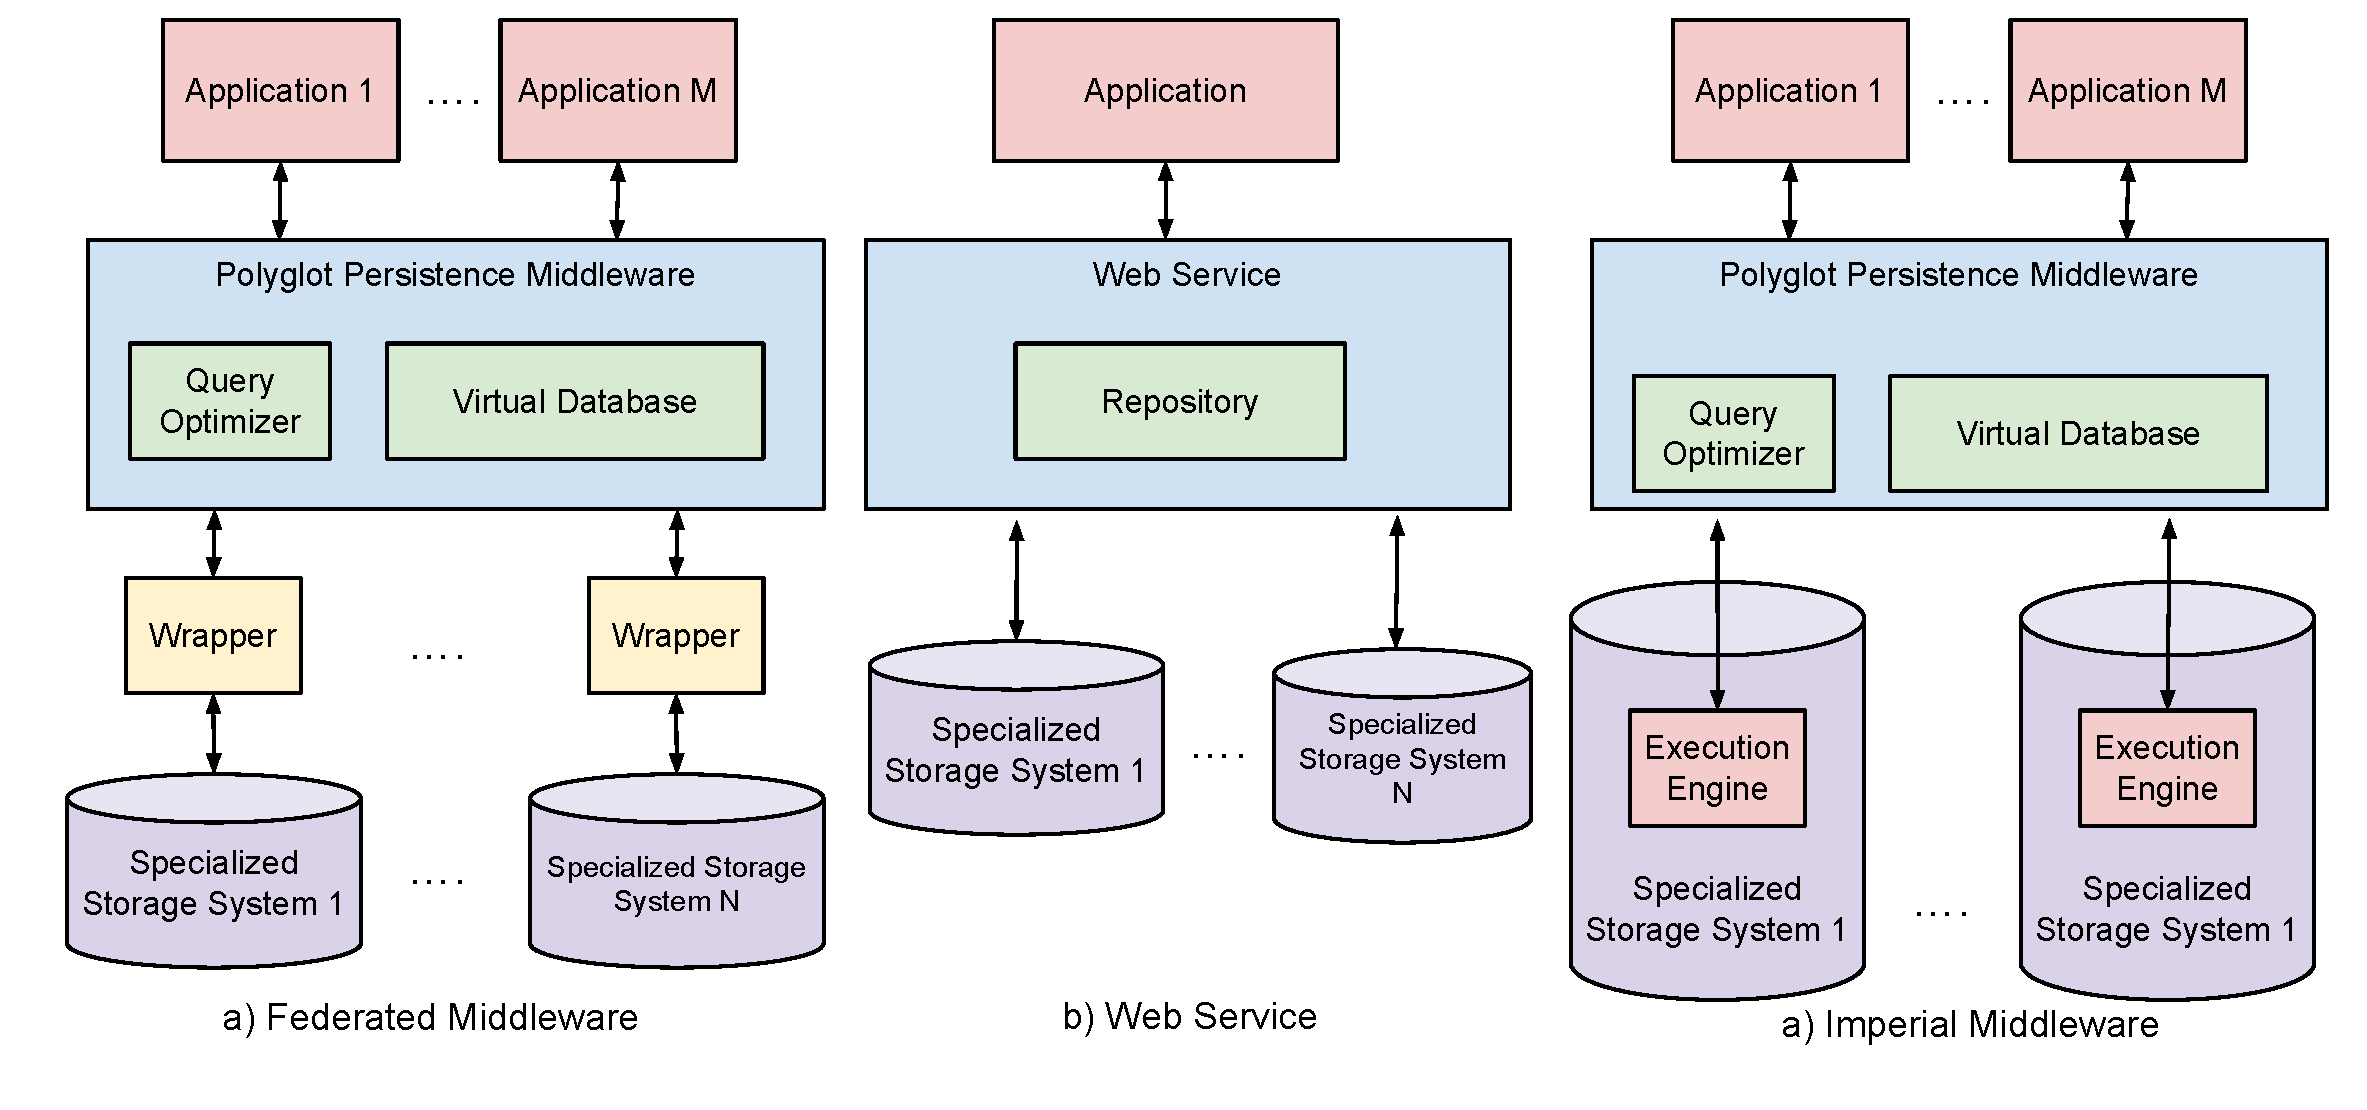
\includegraphics[width=0.8\textwidth]{images/MiddlewareArchitecture.pdf}
  \caption{Classical Middleware Data Integration Architecture applied to our running example}
  \label{fig:dblandscape}
\end{figure}



